\documentclass[12pt]{article}
\usepackage{graphicx} % Required for inserting images
\usepackage[font=small,labelfont=bf]{caption} % Required for specifying captions to tables and figures
\usepackage{fullpage}
\usepackage{clrscode3e}
\usepackage{amsthm,amsmath,amssymb}
\usepackage{mathabx}
\usepackage{xspace}
\usepackage[shortlabels]{enumitem}
\usepackage{caption}
\usepackage{subcaption}
\usepackage{placeins}
\usepackage{listings}
\usepackage{xcolor}
\usepackage{minted}
\usepackage{graphicx}
\usepackage{subcaption}
\usepackage{placeins}   
\newcommand{\code}[1]{\colorbox{gray!20}{\texttt{#1}}}

\title{ENGR 071: Digital Signal Processing\\Lab 1: Aliasing}
\author{Kimaru Boruett}
\date{February 16 2025}

\begin{document}

\maketitle

\section{Introduction}
This lab explores how the sample rate for discrete signals affects the frequency content. If a signal is sampled too slowly, high-frequency components will be aliased into lower frequencies, producing a sampled signal that does not accurately represent the original one. When a signal is sampled, the frequency spectrum becomes a series of periodic spectra, each having a frequency range up to the Nyquist rate, which is half the sampling rate. The purpose of this lab is to experiment with aliasing by subsampling digital music and observing the effects in both the time and frequency domains. Additionally, this lab explores anti-aliasing filters to remove frequency components before subsampling.

\section{Procedure}
The lab was divided into four parts: obtaining music data, conducting aliasing experiments, exploring anti-aliasing filters, and solving a mystery. 
\subsection{Part A - Getting Data}
For this I chose to download \textit{Stay With Me} by Miki Matsubara in mp3 format and used the  \code{audioread} command in MATLAB to read the msuic file into the workspace. I assigned the audio data to the variable \code{music} and the sampling rate to \code{Fs}. I verified the sampling rate and reduced the music file to a single channel since it was originally in stereo, then created a time vector corresponding to the audio data and plotted the signal to visualize it in the time domain. Finally, I reduced the length of the music file to 10s to make it easier to work with and make repeated observations.
\subsection{Part B - Aliasing Experiments}
I conducted aliasing experiments by subsampling the music at various rates, specifically \code{$Fs/5$}, \code{$Fs/15$}, and \code{$Fs/25$}. To subsample, I selected every nth sample using commands like \code{$music\_by\_5 = music(1:5:end)$}. I listened to the original and subsampled music files, noting the changes in sound quality. As the sampling rate decreased, the music sounded increasingly distorted. I generated time-domain plots of the signals and calculated the Fourier transform to analyze the frequency domain characteristics, and generated plots for the same. I used the \code{signalAnalyzer} tool in MATLAB to visualize the power spectra of both the original and subsampled signals. I typed \code{signalAnalyzer} in the MATLAB workspace, dragged the signals into the chart window, and set the time specification to "Sample Rate and Start Time". I displayed multiple signals and spectra by dragging each file name into the time window and entering the corresponding sampling frequency.
\subsection{Part C - Anti Aliasing Filters}
In this part, I explored anti-aliasing filters using the \textit{filterDesigner} tool in MATLAB to design a low-pass filter that removed frequencies that would be aliased during subsampling. I launched the tool by typing \code{filterDesigner} in the MATLAB workspace and set the response type to "\textit{Lowpass}" and the design method to "\textit{FIR Equiripple}". For this I decided to do \code{$Fs/25$} which yields a 1.764 kHz sample rate. I input the original signal's frequency $(44.1kHz)$ in the \textit{Fs box} and specified a value slightly below the Nyquist frequency $(700Hz)$ for the subsampled signal in the Fpass box. I exported the filter coefficients (b's) to the MATLAB workspace, naming the variable "\code{Num}". I filtered the original signal using the \code{filtfilt} command: \code{$music\_filtered = filtfilt(Num, 1, music\_10s);$}. I played the original, filtered, subsampled, and subsampled-filtered music files, and described the differences I observed in the results and discussion section. The filtered music sounded cleaner, with fewer high-frequency artifacts. I analyzed the power spectra of these signals using \textit{signalAnalyzer}.
\subsection{Part D - A Mystery}
I downloaded the "\textit{2001\_a\_space\_oddity.wav}" file and played it in MATLAB using the \code{sound} command. I played the file again, listening to only every 5th sample, revealing a message. I then analyzed the power spectra of these signals using \code{signalAnalyzer}.

\newpage
\section{Results \& Discussion}
\subsection{Part A - Getting Data}
The original sample was 40 seconds long. I cropped it to the first 10 seconds as shown in fig. 1 below for easier and repeated observations.

\begin{figure}[htbp]
  \centering
  \begin{subfigure}[b]{0.48\textwidth} % Adjusted width to fit better
    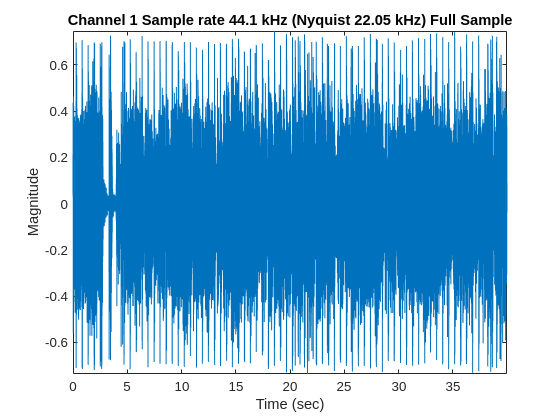
\includegraphics[width=\linewidth]{labs/lab1/lab-report-tex/figures/figure_0.png}
    \caption{Original}
    \label{fig:f1}
  \end{subfigure}
  \hfill
  \begin{subfigure}[b]{0.48\textwidth} % Adjusted width to fit better
    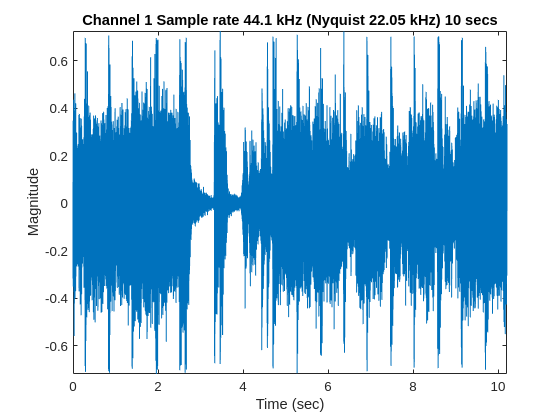
\includegraphics[width=\linewidth]{labs/lab1/lab-report-tex/figures/figure_1.png}
    \caption{Cropped}
    \label{fig:f2}
  \end{subfigure}
  \caption{My flowers.}
\end{figure}
\FloatBarrier

\subsection{Part B - Aliasing Experiments}
\subsubsection{Time-domain Observations}
At \code{$Fs/5$}, the audio remained mostly recognizable, and the overall structure of the music was still clear. However, there was a noticeable reduction in clarity, making the details of certain instruments and tones less defined. The sound felt slightly different, though the main elements including the lyrics of the piece were still easy to follow. At \code{$Fs/15$}, the differences became more pronounced, with the music sounding less distinct and certain parts blending together. The separation between instruments and notes was reduced, making it harder to pick out individual elements. The overall texture of the sound changed, giving it a somewhat flattened quality. By \code{$Fs/25$}, much of the original detail was lost, and the music became difficult to follow. The structure was still present, but it was much harder to recognize specific features of the original piece. Distinguishing between different parts of the music became increasingly challenging.

When examining the time-domain plots below, they appear visually similar across the different sampling rates. This was expected since the overall amplitude envelope of the signal remained intact. However, upon closer inspection, the differences lay in the finer details. Paying attention to the magnitude between \textit{4s} and \textit{8s} will across all the plots will reveal some slight difference. Since the waveform was reconstructed with fewer data points this lead to a loss of smoothness. While these changes were subtle in the time domain, their impact was dramatically evident in the frequency domain outlined next and when playing the sound.
\begin{figure}[htbp]
  \centering
  \begin{subfigure}[b]{0.48\textwidth} % Adjusted width to fit better
    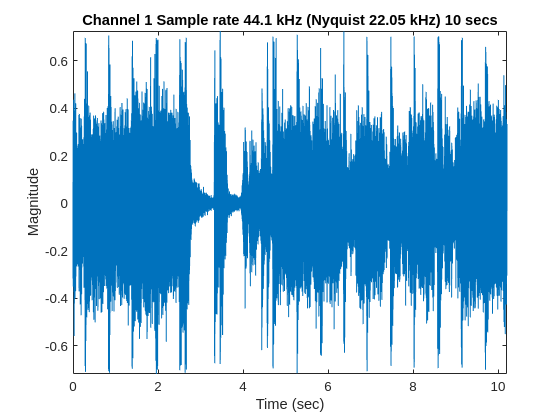
\includegraphics[width=\linewidth]{labs/lab1/lab-report-tex/figures/figure_1.png}
    \caption{44.1kHz}
    \label{fig:f2}
  \end{subfigure}
  \begin{subfigure}[b]{0.48\textwidth} % Adjusted width to fit better
    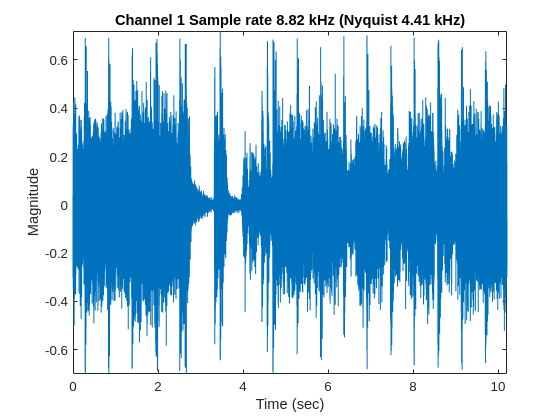
\includegraphics[width=\linewidth]{labs/lab1/lab-report-tex/figures/figure_2.png}
    \caption{8.82kHz}
    \label{fig:f1}
  \end{subfigure}
  \hfill
  \begin{subfigure}[b]{0.48\textwidth} % Adjusted width to fit better
    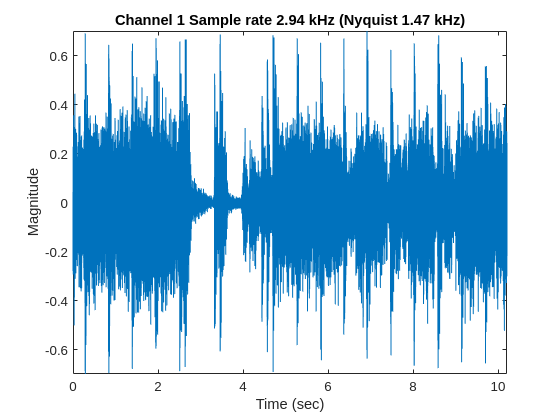
\includegraphics[width=\linewidth]{labs/lab1/lab-report-tex/figures/figure_3.png}
    \caption{2.94kHz}
    \label{fig:f2}
  \end{subfigure}
  \begin{subfigure}[b]{0.48\textwidth} % Adjusted width to fit better
    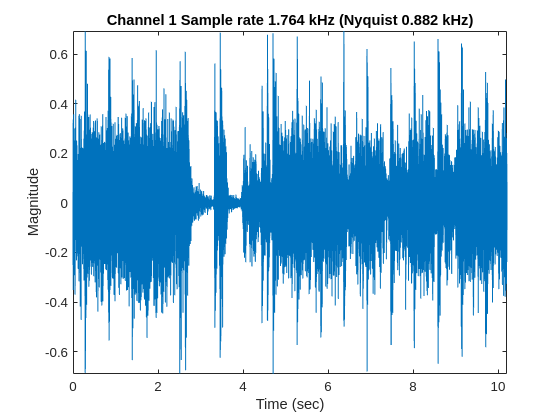
\includegraphics[width=\linewidth]{labs/lab1/lab-report-tex/figures/figure_4.png}
    \caption{1.764kHz}
    \label{fig:f2}
  \end{subfigure}
  \caption{Time-domain representation of the audio signal at different sampling rates (\code{Fs/5, Fs/15, Fs/25, and Fs}). The differences, though subtle in the time domain, significantly impact the perceived audio quality when played back.}
\end{figure}
\FloatBarrier

\subsubsection{Frequency-domain Observations}
Fig. 3 below shows the frequency spectrum of the audio signal sampled at 44.1 kHz, displayed in both linear and decibel (dB) scales. The signal exhibits a concentration of energy in the lower frequencies, predominantly below 5000 Hz. However, there are also noticeable high-frequency components extending towards the Nyquist limit (22.1 kHz), suggesting the presence of harmonics or higher-frequency details. The linear magnitude spectrum highlights the absolute signal strength, while the dB scale provides better insight and reveals lower amplitude components.

\FloatBarrier
\begin{figure}[htbp]
  \centering
  \begin{subfigure}[b]{0.48\textwidth} % Adjusted width to fit better
    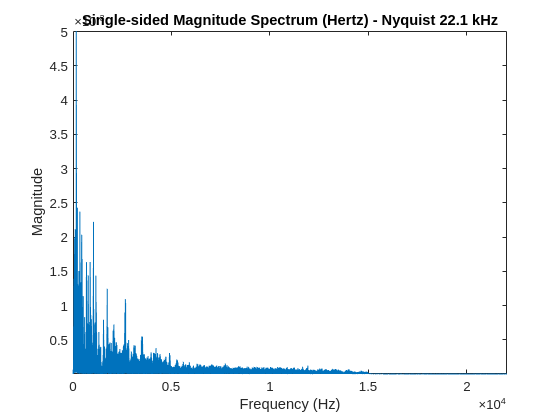
\includegraphics[width=\linewidth]{labs/lab1/lab-report-tex/figures/figure_5.png}
    \caption{Magnitude spectrum in dB scale}
    \label{fig:f2}
  \end{subfigure}
  \begin{subfigure}[b]{0.48\textwidth} % Adjusted width to fit better
    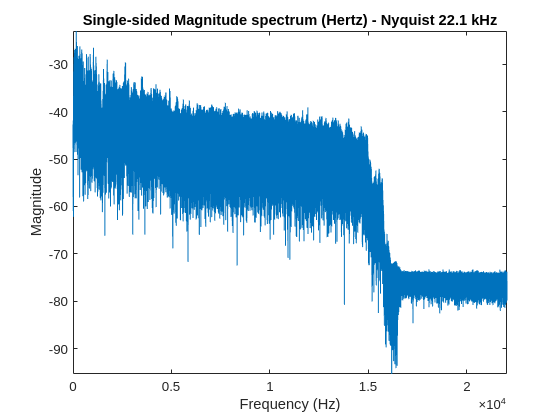
\includegraphics[width=\linewidth]{labs/lab1/lab-report-tex/figures/figure_6.png}
    \caption{Linear magnitude spectrum}
    \label{fig:f1}
  \end{subfigure}
  \caption{Frequency domain representation of the audio signal at a 44.1 kHz sampling rate}
\end{figure}
\FloatBarrier

Fig. 4 below shows the frequency spectrum of the audio signal sampled at 8.82 kHz. The frequency spectrum still retains much of the original structure but with a reduced Nyquist limit. The lower sampling rate restricts the observable frequency range, making it harder to analyze high-frequency components. Since the the original signal contains frequencies higher than the new Nyquist limit, some aliasing must have occurred. The primary low-frequency content however, still remained mostly intact, preserving the core characteristics of the signal.
\FloatBarrier
\begin{figure}[htbp]
  \centering
  \begin{subfigure}[b]{0.48\textwidth} % Adjusted width to fit better
    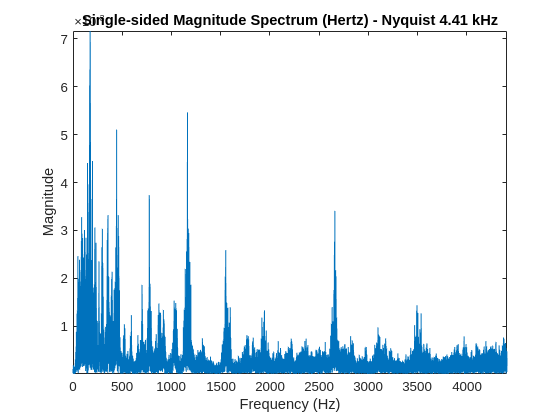
\includegraphics[width=\linewidth]{labs/lab1/lab-report-tex/figures/figure_7.png}
    \caption{Magnitude spectrum in dB scale}
    \label{fig:f2}
  \end{subfigure}
  \begin{subfigure}[b]{0.48\textwidth} % Adjusted width to fit better
    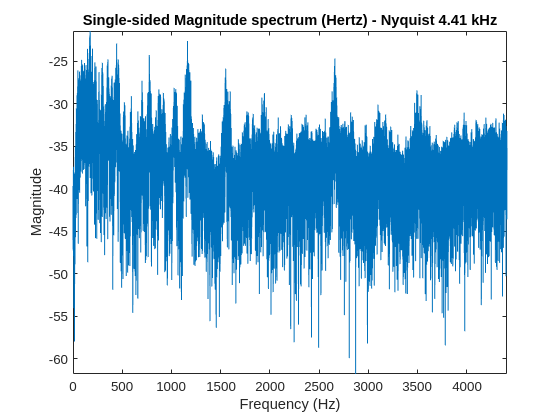
\includegraphics[width=\linewidth]{labs/lab1/lab-report-tex/figures/figure_8.png}
    \caption{Linear magnitude spectrum}
    \label{fig:f2}
  \end{subfigure}
  \caption{Frequency domain representation of the audio signal at a \code{$Fs/5 = 8.82kHz$} sampling rate}
\end{figure}
\FloatBarrier
Fig. 5 below shows the frequency spectrum of the audio signal sampled at 2.94 kHz, giving a Nyquist frequency of 1.47 kHz. The reduction in sampling rate significantly limits the observable frequency range, capturing only the lowest-frequency components of the original signal. Although the primary low-frequency content remains mostly intact, the relatively higher-frequency elements above 1.5 kHz, which were present in the original signal, are now partially lost or distorted due to aliasing. Frequencies above the Nyquist limit fold back into the spectrum, causing unwanted spectral overlap. While some of the original structure can still be seen, the loss of higher frequencies impacts the overall accuracy, making it harder to analyze certain features of the signal.

\FloatBarrier
\begin{figure}[htbp]
  \centering
  \begin{subfigure}[b]{0.48\textwidth} % Adjusted width to fit better
    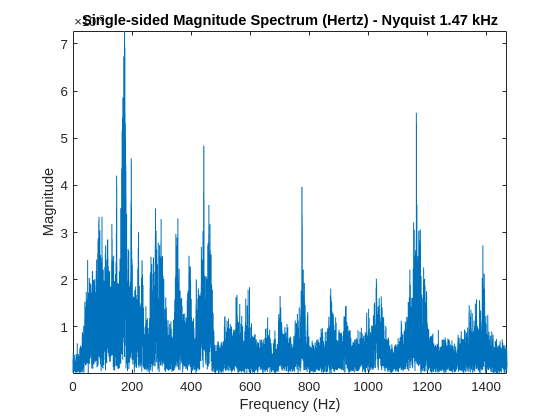
\includegraphics[width=\linewidth]{labs/lab1/lab-report-tex/figures/figure_9.png}
    \caption{Magnitude spectrum in dB scale}
    \label{fig:f2}
  \end{subfigure}
  \begin{subfigure}[b]{0.48\textwidth} % Adjusted width to fit better
    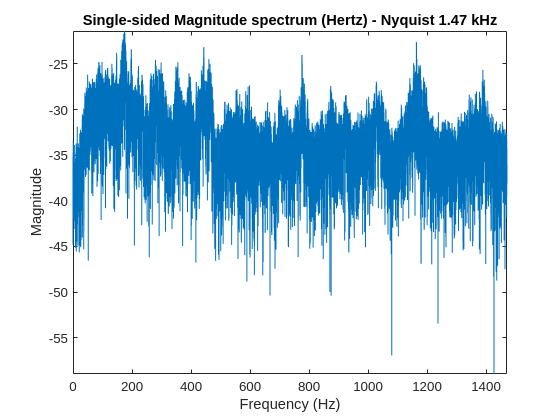
\includegraphics[width=\linewidth]{labs/lab1/lab-report-tex/figures/figure_10.png}
    \caption{Linear magnitude spectrum}
    \label{fig:f2}
  \end{subfigure}
  \caption{Frequency domain representation of the audio signal at a \code{$Fs/15 = 2.94kHz$} sampling rate}
\end{figure}
\FloatBarrier
Fig. 6 below shows the frequency spectrum of the audio signal sampled at 1.764 kHz, giving a Nyquist frequency of 0.882 kHz. This sampling rate severely limits the range of frequencies that can be accurately represented. The original signal contained important high-frequency components above 1 kHz, but since they exceed the Nyquist limit, they are aliased back into the lower spectrum, significantly distorting the signal’s frequency content. As a result, the spectrum is dominated by incorrect frequency components, making it difficult to distinguish the original characteristics of the signal. The primary low-frequency content below 880 Hz is still present, but the higher-frequency details are irreversibly lost or misrepresented, reducing the fidelity of the sampled signal.


\begin{figure}[htbp]
  \centering
  \begin{subfigure}[b]{0.48\textwidth} % Adjusted width to fit better
    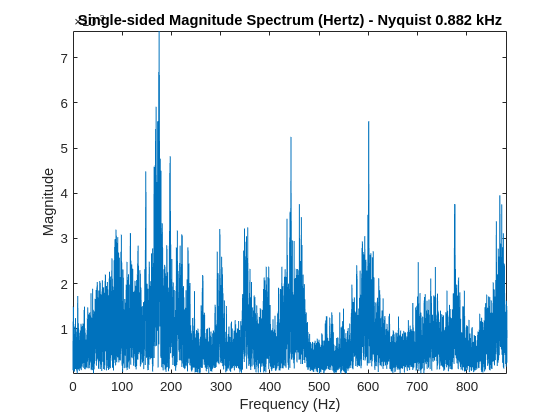
\includegraphics[width=\linewidth]{labs/lab1/lab-report-tex/figures/figure_11.png}
    \caption{Magnitude spectrum in dB scale}
    \label{fig:f2}
  \end{subfigure}
  \begin{subfigure}[b]{0.48\textwidth} % Adjusted width to fit better
    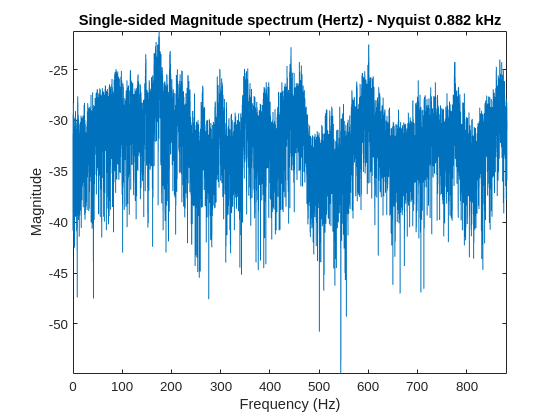
\includegraphics[width=\linewidth]{labs/lab1/lab-report-tex/figures/figure_12.png}
    \caption{Linear magnitude spectrum}
    \label{fig:f2}
  \end{subfigure}
  \caption{Frequency domain representation of the audio signal at a \code{$Fs/25 = 1.764kHz$} sampling rate}
\end{figure}
\FloatBarrier
Fig. 7 below shows the power spectrum analysis of the signals at different sampling rates reveals the effects of reduced sampling on frequency representation. In the time domain, slight differences can be observed, particularly as the sampling rate decreases. At 8.82 kHz, the sampled signal closely follows the original, with minimal distortion. However, in the frequency domain, aliasing is noticeable as some frequency components appear to have magnitudes equal to or greater than those of the original signal. This suggests spectral overlap, where aliased frequencies reinforce existing components rather than fully distorting them.

As the sampling rate is further reduced to 2.94 kHz, the effects of aliasing become more pronounced. The time-domain representation shows a loss of fine details, and in the frequency domain, more spectral components are folded back into the lower frequencies, altering the overall structure of the spectrum. At 1.764 kHz, the lowest sampling rate, aliasing is the most severe, completely distorting the spectral content. Frequencies beyond the Nyquist limit are heavily folded back, making the original frequency distribution almost unrecognizable.

Fig. 7(d) presents all signals together, making it easier to compare their spectral differences. When viewed side by side, it becomes clear that the signal sampled at 1.764 kHz has the greatest aliasing, with significant spectral overlap and distortion. The comparison highlights the importance of selecting an appropriate sampling rate to maintain the integrity of the original signal while avoiding aliasing artifacts.

\begin{figure}[htbp]
  \centering
  \begin{subfigure}[b]{0.48\textwidth} % Adjusted width to fit better
    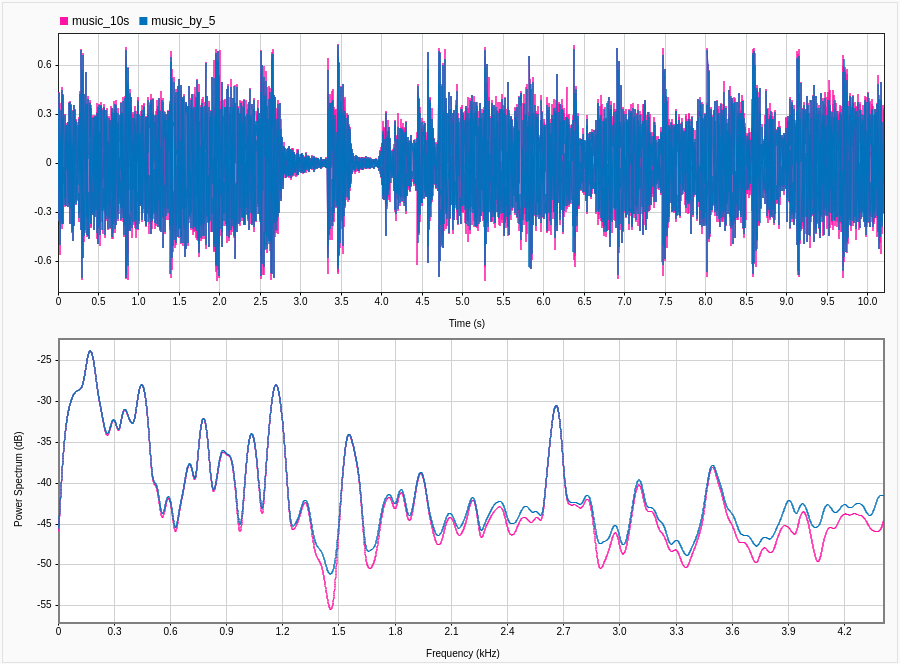
\includegraphics[width=\linewidth]{labs/lab1/lab-report-tex/figures/SigAnalyzer/part B/orig_by5.png}
    \caption{Original and 8.82 kHz}
    \label{fig:f2}
  \end{subfigure}
  \begin{subfigure}[b]{0.48\textwidth} % Adjusted width to fit better
    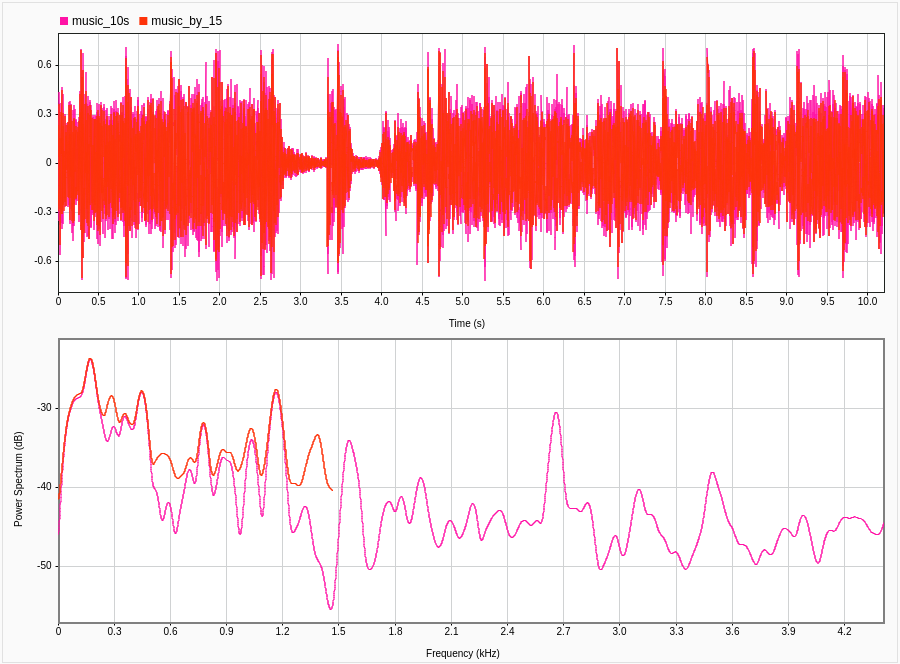
\includegraphics[width=\linewidth]{labs/lab1/lab-report-tex/figures/SigAnalyzer/part B/orig_by15.png}
    \caption{Original and 2.94 kHz}
    \label{fig:f2}
  \end{subfigure}
  \begin{subfigure}[b]{0.48\textwidth} % Adjusted width to fit better
    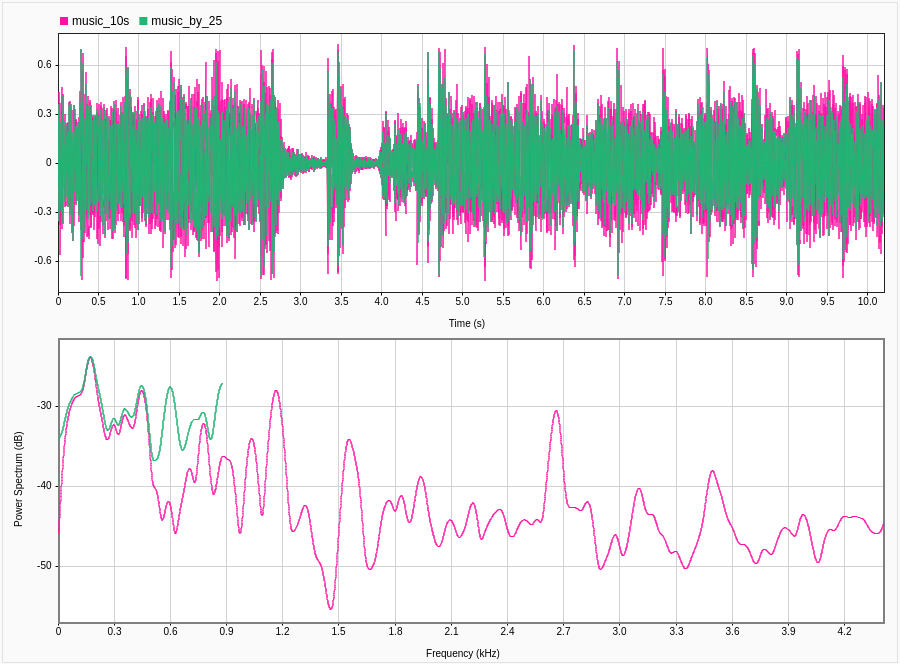
\includegraphics[width=\linewidth]{labs/lab1/lab-report-tex/figures/SigAnalyzer/part B/orig_by25.png}
    \caption{Original and 1.764kHz}
    \label{fig:f2}
  \end{subfigure}
  \begin{subfigure}[b]{0.48\textwidth} % Adjusted width to fit better
    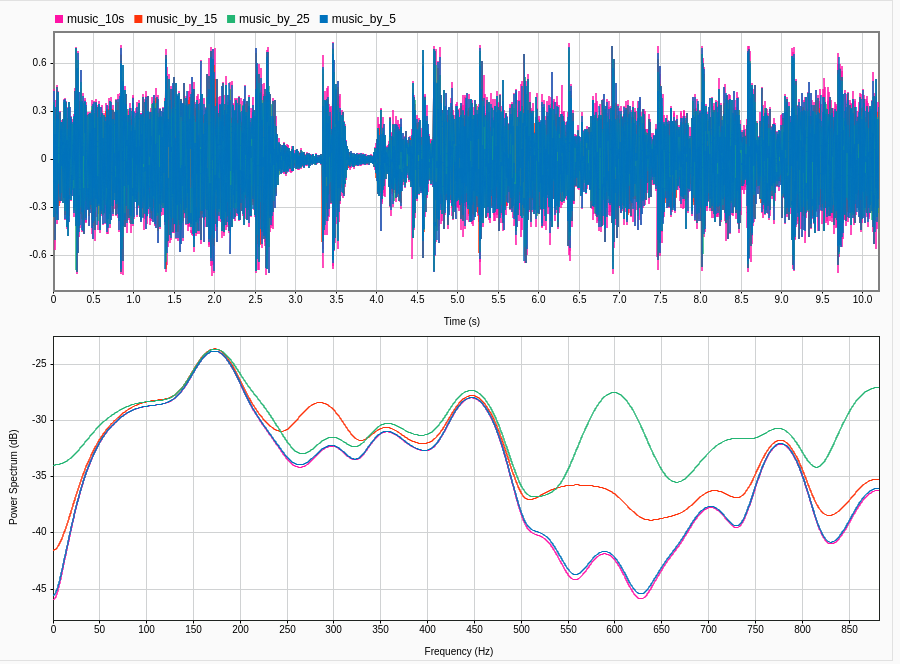
\includegraphics[width=\linewidth]{labs/lab1/lab-report-tex/figures/SigAnalyzer/part B/all.png}
    \caption{All signals}
    \label{fig:f2}
  \end{subfigure}
  \caption{Time and frequency domain representations of the original audio signal and its sampled versions at different rates, generated using \code{signalAnalyzer}}
\end{figure}
\FloatBarrier
\subsection{Part C - Anti Aliasing Filters}
Before applying the anti-aliasing filter, the audio signal sampled at 1.764 kHz suffered from severe aliasing, making the lyrics unintelligible and the music distorted. High-frequency components folded back into the lower spectrum, creating unnatural artifacts that blurred the distinction between instruments and affected the clarity of the sound. After filtering with a 700 Hz cutoff, the clarity improved significantly. The lyrics became intelligible, and the music sounded more natural, with fewer distortions affecting its harmonic structure. By removing the frequencies that would have caused aliasing, the filtered version preserved the essential low-frequency content, maintaining the rhythm and melody without unnatural interference. While some high-frequency details were lost, the overall listening experience was much clearer.

Fig. 8(a) presents the original signal alongside its filtered counterpart before being sampled at 1.764 kHz. Given the Nyquist frequency of 882 Hz, the filter is designed with a passband cutoff at 700 Hz and a stopband beginning at 900 Hz to effectively remove frequency components that could lead to aliasing. This is evident in the filtered spectrum, where frequency content above 700 Hz gradually diminishes, and by 850 Hz, the signal power is significantly reduced.

Fig. 8(b) compares the original signal with the version obtained after sampling the filtered signal. The two signals exhibit a high correlation, with their time-domain waveforms closely matching. However, differences become noticeable beyond the 700 Hz cutoff, where the filtered signal loses higher-frequency components. This confirms the effectiveness of the anti-aliasing filter in preserving the original structure while eliminating frequencies that could cause aliasing when sampled at 1.764 kHz.
\FloatBarrier
\begin{figure}[htbp]
  \centering
  \begin{subfigure}[b]{0.48\textwidth} % Adjusted width to fit better
    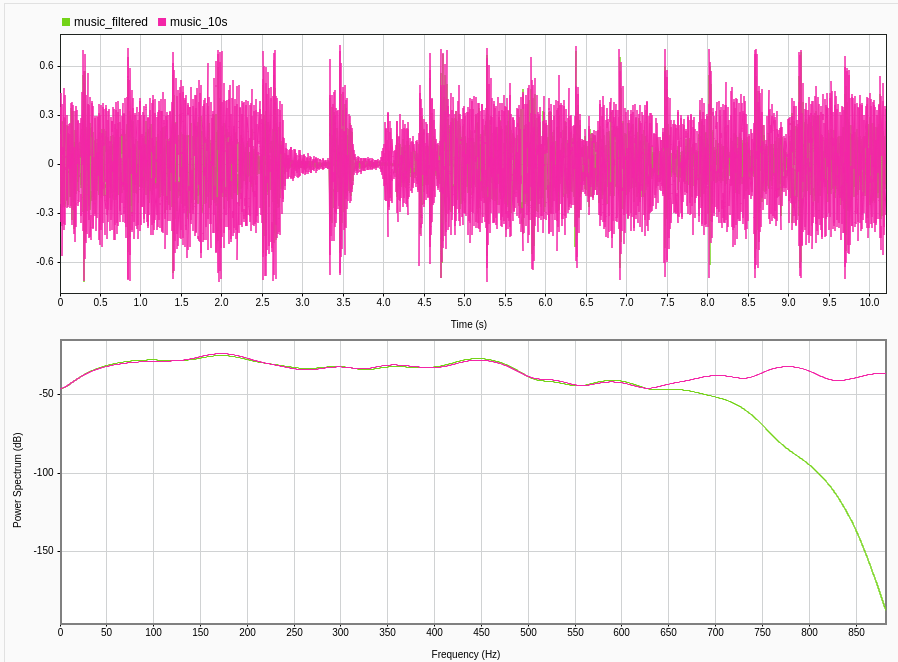
\includegraphics[width=\linewidth]{labs/lab1/lab-report-tex/figures/SigAnalyzer/PArt C/ps_mus_filt_orig.png}
    \caption{Original and filtered signals, showing attenuation of frequencies above 700 Hz.}
    \label{fig:f2}
  \end{subfigure}
  \begin{subfigure}[b]{0.48\textwidth} % Adjusted width to fit better
    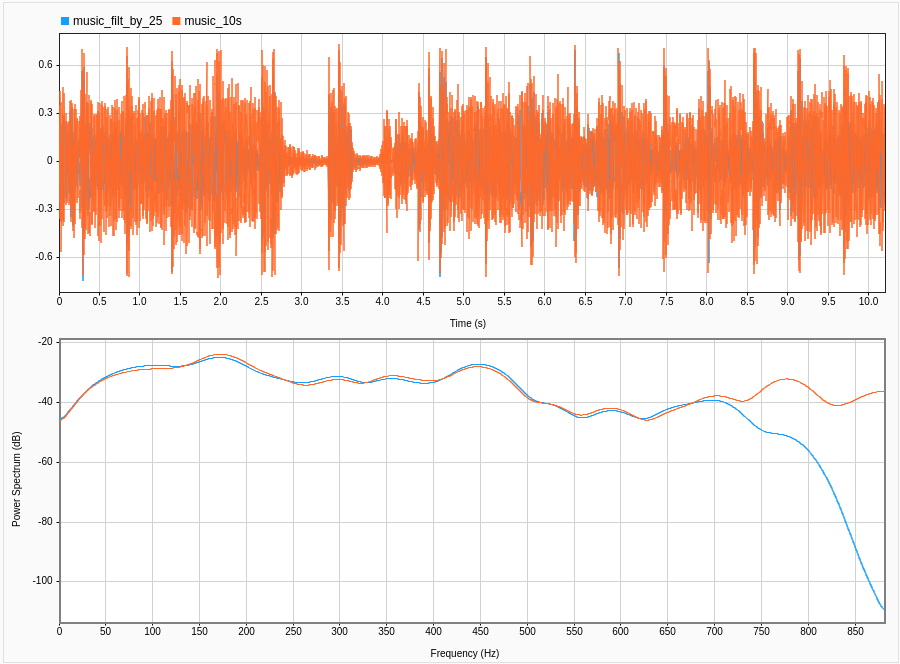
\includegraphics[width=\linewidth]{labs/lab1/lab-report-tex/figures/SigAnalyzer/PArt C/filt25_origi.png}
    \caption{Original signal compared to the filtered version at 1764 Hz}
    \label{fig:f2}
  \end{subfigure}
  \caption{Comparison of the original and filtered audio signals}
\end{figure}
\FloatBarrier
Fig. 9(a) below compares the filtered signal to its subsampled version at 1.764 kHz, demonstrating that the filtering process successfully eliminated high-frequency components that would have caused aliasing. The two signals are nearly indistinguishable, confirming that the Nyquist limit (882 Hz) is within the lowest frequency content retained in the signal. Because the filtering removed frequencies beyond the Nyquist rate before sampling, the subsampled version accurately preserves the structure of the original filtered signal. This ensures that no aliasing artifacts appear, making the sampled version a decent representation of the input.

Fig. 9(b) compares all signals, including one sampled at 1.764 kHz without filtering. This unfiltered version contains frequency components beyond the Nyquist limit, leading to aliasing that distorts the frequency representation. Unlike the filtered version, which closely matches the original up to the 700 Hz cutoff, the unfiltered sample exhibits aliasing artifacts even around 500 Hz, showing how high-frequency elements have folded back into the spectrum. This distortion alters the spectral structure, making it differ significantly from the original signal. 
\FloatBarrier
\begin{figure}[htbp]
  \centering
  \begin{subfigure}[b]{0.48\textwidth} % Adjusted width to fit better
    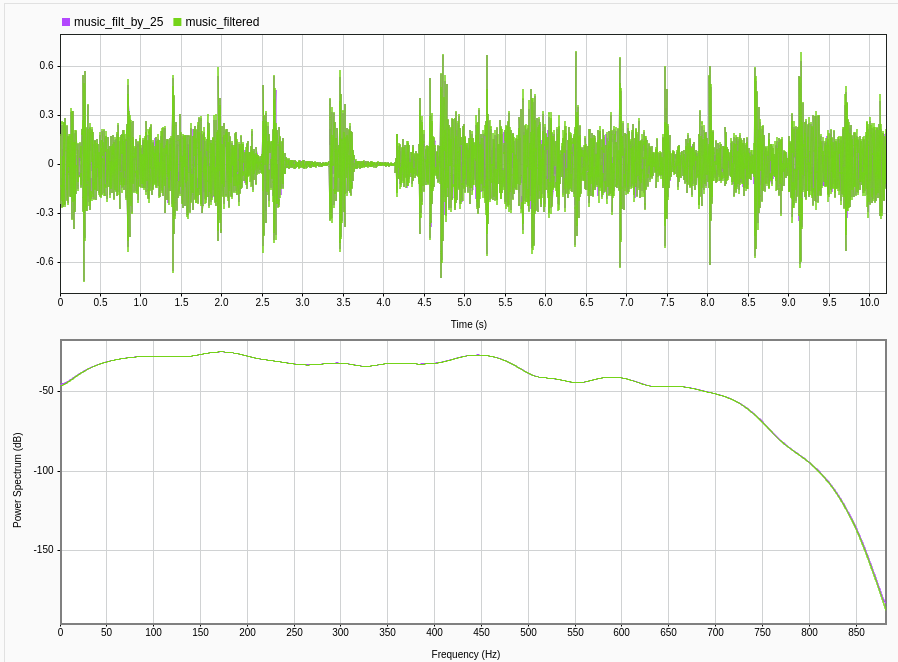
\includegraphics[width=\linewidth]{labs/lab1/lab-report-tex/figures/SigAnalyzer/PArt C/ps_filt25_filt.png}
    \caption{Filtered and 1.764 kHz sampling of Filtered}
    \label{fig:f2}
  \end{subfigure}
  \begin{subfigure}[b]{0.48\textwidth} % Adjusted width to fit better
    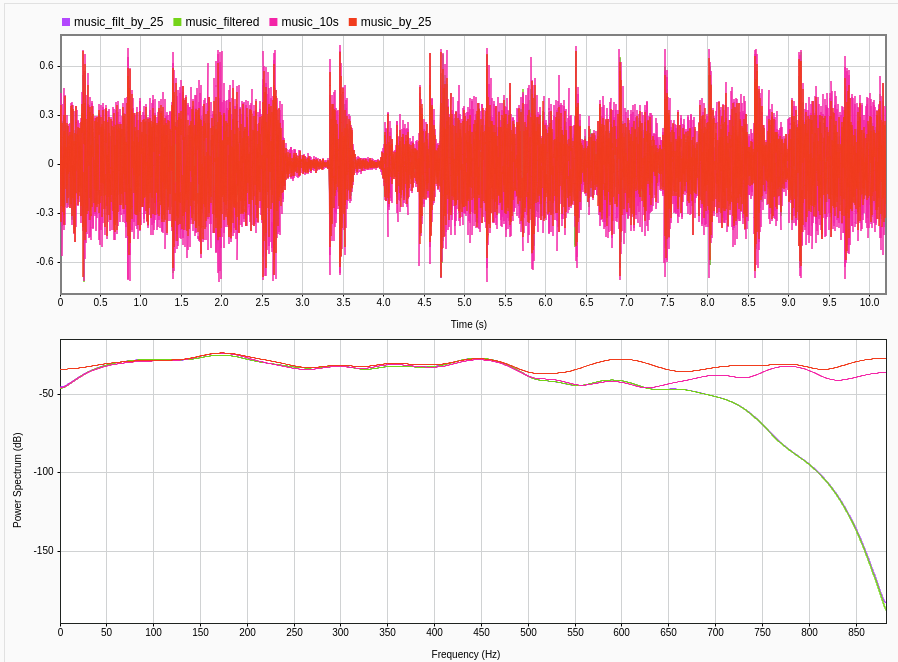
\includegraphics[width=\linewidth]{labs/lab1/lab-report-tex/figures/SigAnalyzer/PArt C/ps_all_signals_filt.png}
    \caption{All signals including 1.76kHz sampling before filtering}
    \label{fig:f2}
  \end{subfigure}
  \caption{Effects of anti-aliasing filtering before sampling at 1.764 kHz}
\end{figure}
\FloatBarrier

\subsection{Part D - A Mystery}
When the signal containing original was sampled at 8.82 kHz, aliasing altered its spectral content in a way that revealed speech that was previously masked. In the original signal, strong frequency components above 15 kHz obscured the speech, making it unintelligible. However, after sampling, the Nyquist limit was reduced to 4.41 kHz, meaning that all frequency content above this threshold either folded back into the lower frequencies or was removed. This aliasing effect resulted in a redistribution of spectral energy, unintentionally shifting the speech components into an audible range, unraveling the mystery.

As seen in Fig. 10(a) below, the original signal contained a significant amount of high-frequency content above 15 kHz, which dominated the spectrum. After sampling at 8.82 kHz, the frequency spectrum in Fig. 10(b) showed that all information above 4.41 kHz was removed or aliased. Comparing the time-domain representations in Fig. 10(c), subtle differences between the original and sampled signals were evident, indicating changes in signal structure. In the frequency domain, distinct spectral differences appeared after 4.2 kHz, confirming that aliasing reconstructed the speech components that were otherwise masked in the original signal. 
\FloatBarrier
\begin{figure}[htbp]
  \centering
  \begin{subfigure}[b]{0.48\textwidth} % Adjusted width to fit better
    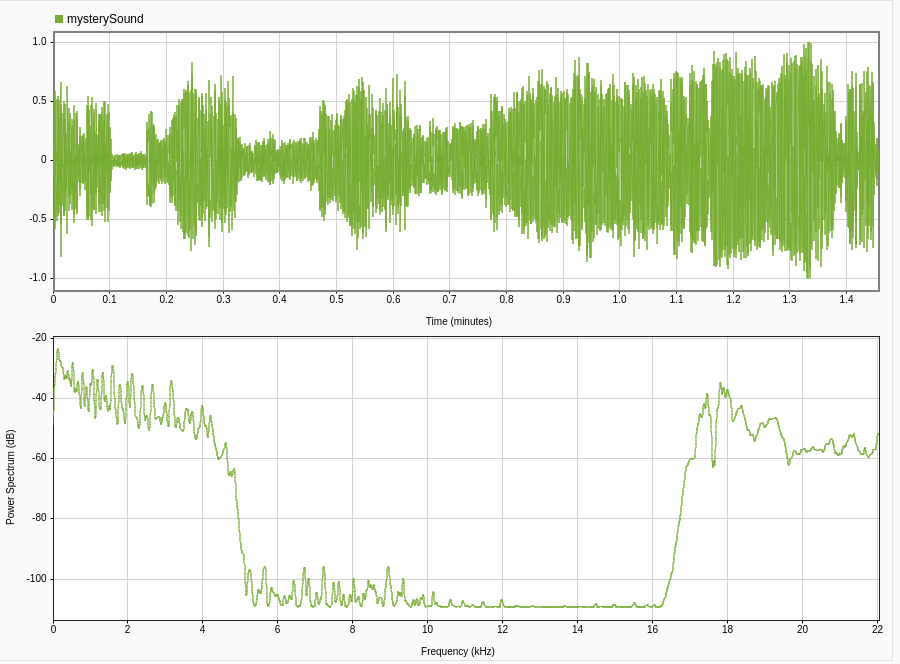
\includegraphics[width=\linewidth]{labs/lab1/lab-report-tex/figures/SigAnalyzer/PartD/mystery.png}
    \caption{Original Sampled at 44.1 kHz}
    \label{fig:f2}
  \end{subfigure}
  \begin{subfigure}[b]{0.48\textwidth} % Adjusted width to fit better
    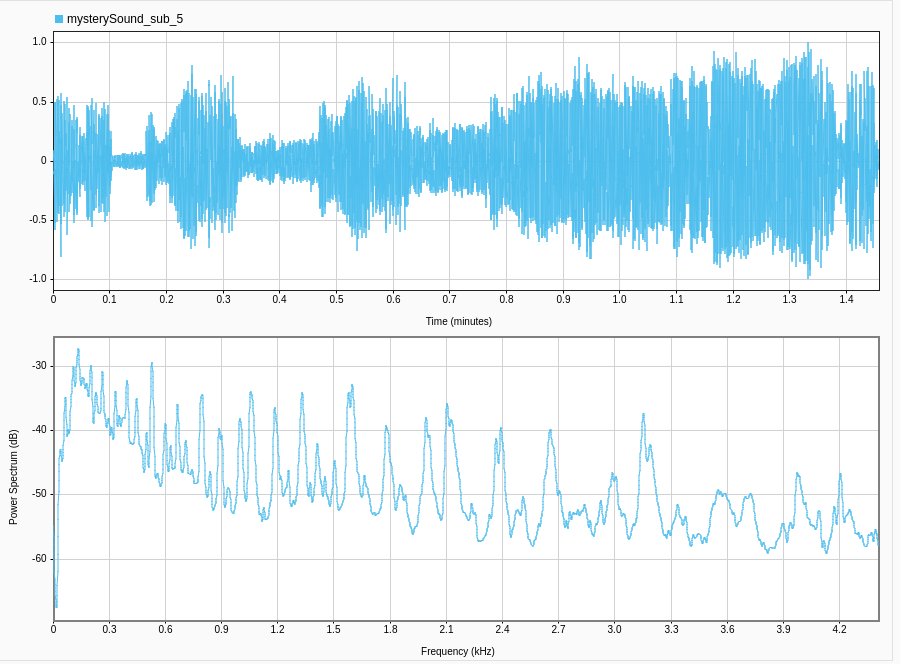
\includegraphics[width=\linewidth]{labs/lab1/lab-report-tex/figures/SigAnalyzer/PartD/mystery_by5.png}
    \caption{Sampled at 8.82 kHz}
    \label{fig:f2}
  \end{subfigure}
  \begin{subfigure}[b]{0.48\textwidth} % Adjusted width to fit better
    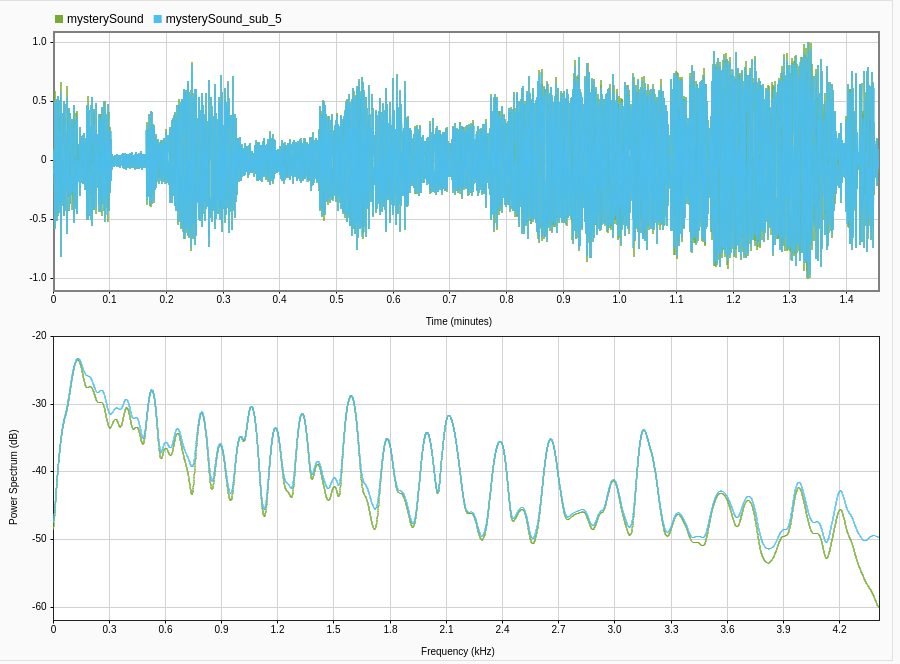
\includegraphics[width=\linewidth]{labs/lab1/lab-report-tex/figures/SigAnalyzer/PartD/both.png}
    \caption{Both signals combined}
    \label{fig:f2}
  \end{subfigure}
  \caption{Observation of aliasing revealing speech content in a signal sampled at 8.82 kHz.}
\end{figure}
\FloatBarrier
\section{Conclusion}
This lab demonstrated the effects of aliasing, the role of anti-aliasing filters, and the importance of frequency domain analysis in understanding sampled signals. Aliasing occurs when a signal is sampled at a rate below twice its highest frequency component, violating the Nyquist criterion and causing high-frequency content to fold back into the lower spectrum. This can distort the original signal, as seen when sampling without pre-filtering. However, in some cases, aliasing can also reveal hidden information, as observed when high-frequency components originally masked speech but were shifted into an audible range after sampling.

The use of anti-aliasing filters before sampling was shown to be effective in preventing spectral distortion. By applying a low-pass filter with a cutoff frequency below the Nyquist limit, unwanted high-frequency components were removed before sampling, ensuring that the signal remained undistorted. This approach preserved the essential characteristics of the original signal while preventing the introduction of misleading spectral artifacts.

Throughout the lab, frequency domain analysis proved to be more informative than time domain analysis. While time-domain representations provided a general view of the signal’s structure, the frequency domain revealed critical details about spectral content, aliasing effects, and filter performance. Observing the power spectrum helped identify regions where aliasing was present and confirmed how filtering shaped the frequency response of the sampled signals. These findings emphasize the importance of proper sampling techniques and spectral analysis in signal processing, ensuring that signals are accurately captured and free from unintended distortions.

\end{document}